% !TEX TS-program = xeLaTeX+MakeIndex+BibTeX 
\documentclass[xcolor=x11names,compress]{ctexbeamer}

\usetheme{Darmstadt} 

\usepackage{multicol}
\usepackage{xeCJK}
\usepackage{fontspec} 

\usepackage{array, booktabs}
\usepackage{graphicx}
\usepackage[x11names]{xcolor}
\usepackage{colortbl}
\definecolor{baseD}{HTML}{7CAFC2}
\newcommand{\timeline}{\color{baseD}\makebox[0pt]{\textbullet}\hskip-0.5pt\vrule width 1pt\hspace{\labelsep}}

\setCJKmainfont[BoldFont=Heiti SC Medium]{PingFang SC}
\setCJKsansfont[BoldFont=Heiti SC Medium]{Kaiti SC}
\setsansfont{Helvetica}
\setmonofont{Menlo}

\setbeamercolor*{lower separation line head}{bg=DeepSkyBlue4} 
\setbeamercolor*{normal text}{fg=black,bg=white}
\setbeamercolor*{alerted text}{fg=red} 
\setbeamercolor*{example text}{fg=black} 
\setbeamercolor*{structure}{fg=DeepSkyBlue4,bg=white} 

\setbeamerfont{block title}{size=\tiny}
\setbeamerfont{block body}{size=\tiny}
\setbeamerfont{block title example}{size=\tiny}
\setbeamerfont{block body alerted}{size=\tiny}
\setbeamerfont{block body example}{size=\tiny}


\setbeamercolor*{palette tertiary}{fg=black,bg=black!10} 
\setbeamercolor*{palette quaternary}{fg=black,bg=black!10} 

%footline
\setbeamercolor{author in head/foot}{fg=white,bg=}
\setbeamercolor{title in head/foot}{fg=white,bg=}
\setbeamercolor{date in head/foot}{fg=black,bg=}


\makeatletter
\setbeamertemplate{footline}
{%
    \setbox\beamer@tempbox=\hbox{%
        \begin{beamercolorbox}[wd=.333333\paperwidth,ht=2.25ex,dp=1ex,center]{author in head/foot}%
            \usebeamerfont{author in head/foot}\insertshorttitle
        \end{beamercolorbox}%
        \begin{beamercolorbox}[wd=.333333\paperwidth,ht=2.25ex,dp=1ex,center]{title in head/foot}%
            \usebeamerfont{title in head/foot}\insertsubsection
        \end{beamercolorbox}%
        \begin{beamercolorbox}[wd=.333333\paperwidth,ht=2.25ex,dp=1ex,right]{date in head/foot}%
            \usebeamerfont{date in head/foot}\insertshortdate{}\hspace*{2em}
            \insertframenumber{} / \inserttotalframenumber\hspace*{2ex} 
        \end{beamercolorbox}%
    }%
    \vskip1.8\baselineskip
        \begin{pgfpicture}{0pt}{0pt}{\paperwidth}{0cm}%
            \usebeamercolor{frametitle right}%
            \pgfpathrectangle{\pgfpointorigin}{\pgfpoint{\paperwidth}{3.5ex}}%
            \pgfusepath{clip}%
            \pgftext[left,base]{\pgfuseshading{beamer@frametitleshade}}%
        \end{pgfpicture}%
    \beamer@tempdim=\ht\beamer@tempbox%
    \advance\beamer@tempdim by 0.95ex%
    \vskip-\beamer@tempdim%
    \box\beamer@tempbox%
}  
\makeatother

\makeatletter
\setbeamertemplate{section page}
{
  \begin{beamercolorbox}[sep=12pt,center]{section title}
    \usebeamerfont{section title}\insertsection\par
  \end{beamercolorbox}
}
\makeatother

\makeatletter
\setbeamertemplate{subsection page}
{
  \begin{beamercolorbox}[sep=8pt,center]{subsection title}
    \usebeamerfont{subsection title}\insertsubsection\par
  \end{beamercolorbox}
}
\makeatother

\AtBeginSection{\frame{\sectionpage}}
\AtBeginSubsection{\frame{\subsectionpage}}

\setbeamertemplate{headline}[default]
\setbeamertemplate{navigation symbols}{}

\colorlet{titleright}{yellow!10!white}
\colorlet{titleleft}{DeepSkyBlue4}
\colorlet{titlemid}{green!60!blue}

\makeatletter

\pgfdeclarehorizontalshading[titleleft,titleright]{beamer@frametitleshade}{\paperheight}{%
        color(0pt)=(titleleft);
        color(.5\paperwidth)=(titlemid);
        color(\paperwidth)=(titleright)
}

\AtBeginDocument{
    \pgfdeclareverticalshading{beamer@topshade}{\paperwidth}{%
        color(0pt)=(bg);
        color(4pt)=(black!50!bg)    
    }
}

\renewcommand{\(}{\begin{columns}}
\renewcommand{\)}{\end{columns}}
\newcommand{\<}[1]{\begin{column}{#1}}
\renewcommand{\>}{\end{column}}

\usepackage[cache=false,outputdir=.texpadtmp]{minted}
\newminted{java}{fontsize=\scriptsize, 
                   linenos,autogobble,breaklines,
                   frame=lines,framesep=8pt
                   } 
\newmint{java}{}
\newmintinline{java}{}



\title{Java编程技术}

\author{徐行健}
 
\institute
{
  计算机与信息工程学院\\
  内蒙古师范大学
}

\date{\today}

\begin{document}

\maketitle

\begin{frame}[t]
  \frametitle{目录}
    \begin{multicols}{2}
      \tableofcontents
    \end{multicols}
\end{frame}

\section[第一部分:导论]{第一部分:导论}
\subsection[第一章:概述]{第一章:概述}
\begin{frame}
  \frametitle{课程介绍}
  \begin{itemize}
    \item Java是一门\textbf{非常重要}的课程,以后很多同学的毕业设计乃至工作都会使用到Java
    \item C/C++ 没学好,不代表你学不好Java!与前两者相比,这是一门相对“简单”的语言
    \item 数据结构没学好,不代表你学不好Java!本课程\textbf{偏向工程应用},很少涉及纯粹的算法
    \item 本课程包含绝大部分Java的基础知识,不包含Web相关内容
  \end{itemize}
\end{frame}

\begin{frame}
  \frametitle{课程要求}
  \begin{itemize}
    \item 实验课代码自己敲,不要复制粘贴!只会照着书或者PPT敲代码的,最后肯定学不好本课程!
    \item 作业算做实验课成绩。作业会有自动查重,不管谁抄谁,所有重复者作业(重复率大于70\%)一律0分!
    \item 本课程不设所谓的及格率下限!考试作弊者重修从严处理!大四清考按照正常出卷和判卷标准执行!
  \end{itemize}
  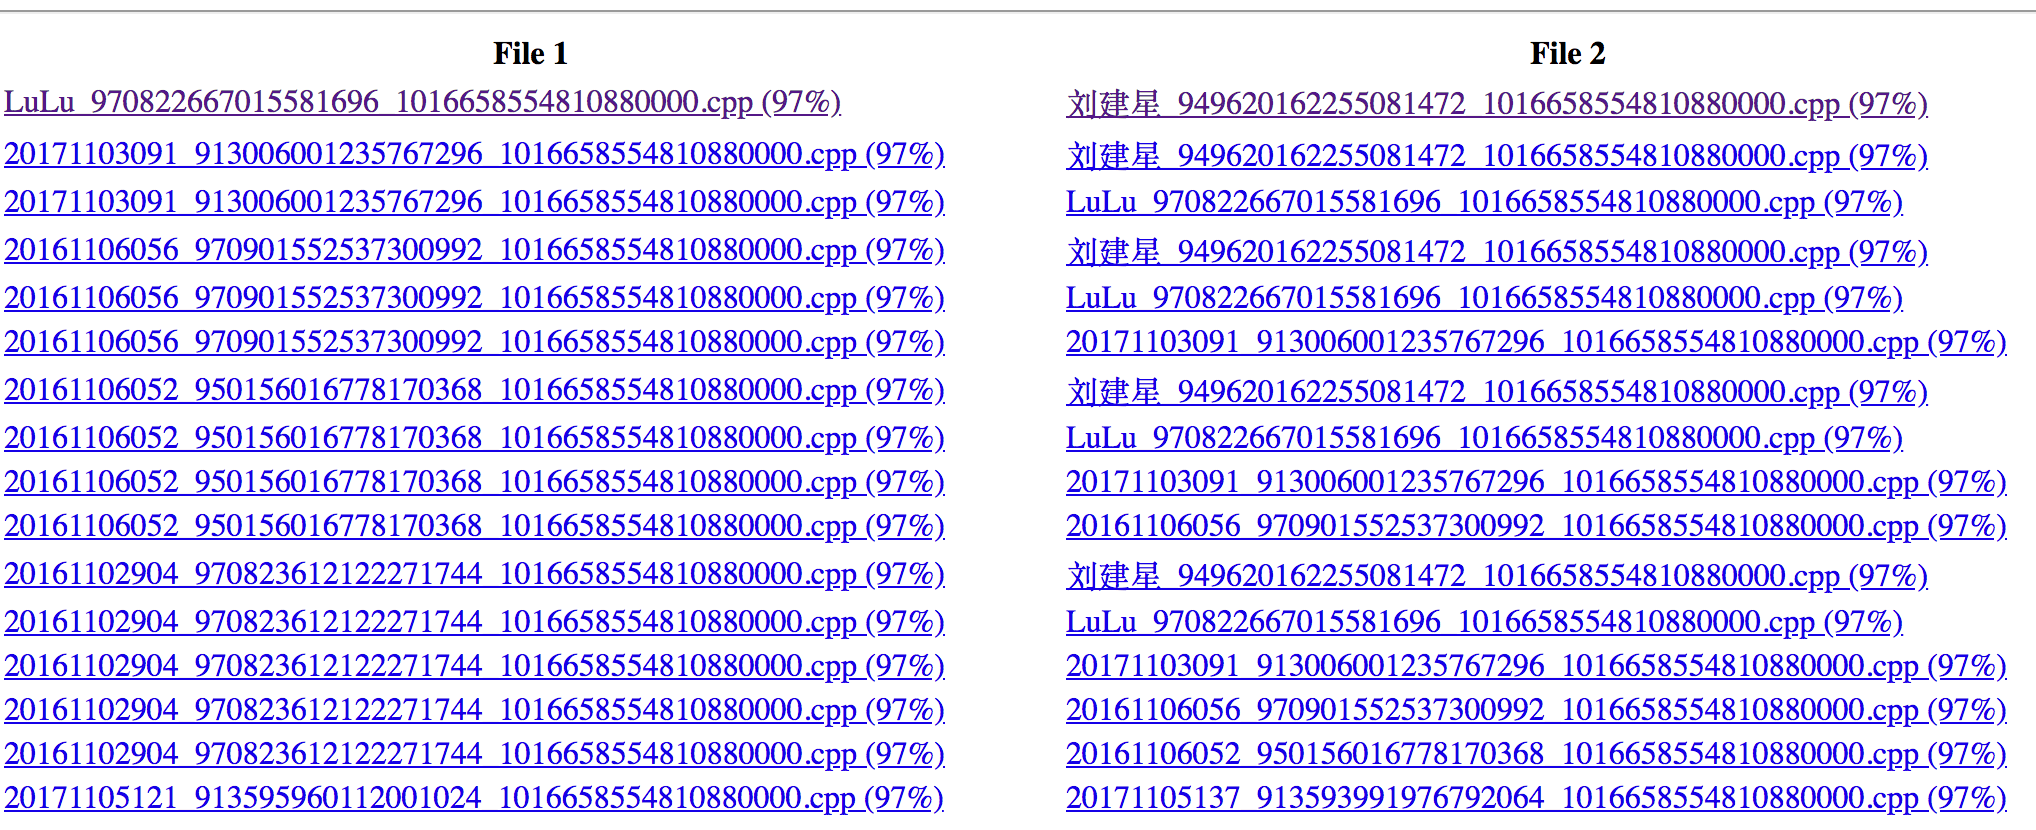
\includegraphics[width=\textwidth]{figures/moss}
\end{frame}


\begin{frame}
  \frametitle{Java语言的历史地位}
  \begin{enumerate}
    \item 第一代语言:打孔机,纯粹的机器语言,易于机器理解和执行。程序员需要掌握全部的硬件细节
    \item 第二代语言:汇编语言,比第一代语言更加容易编写,用抽象的符号表示指令、数据和寄存器,程序员需要掌握大量的硬件细节
    \item 第三代语言:高级语言,易于人类设计程序,对大部分硬件做了抽象
      \begin{itemize}
        \item 分类标准一:
          \begin{itemize}
            \item 面向过程的语言:C、Fortran、Pascal
            \item 不纯粹的面向对象的语言:C++
            \item 纯粹的面向对象的语言:Java
            \item 函数式语言:Lisp
          \end{itemize}
        \item 分类标准二:
          \begin{itemize}
            \item 编译型语言:C、C++、Java
            \item 解释型语言:Python、Javascript、Perl、PHP
          \end{itemize}
      \end{itemize}
  \end{enumerate}
  
  Java和Javascript是两种完全不同、毫无关系的语言!

\end{frame}

\begin{frame}
  \frametitle{Java语言的优点}
  \begin{itemize}
    \item “纯粹”的面向对象:不像C++那样包含过程化编程语言的要素
    \item 跨平台:通过Java虚拟机(JVM)实现了\textbf{平台无关性} ,一次编译,到处运行(write once, run everywhere)
    \item 开发效率高:易于编写、易于调试,易于团队合作,更加适合大型软件项目
    \item 健壮:吸收了C/C++的优点,同时去掉了其不太健壮的部分(如指针,内存的申请和释放),很大程度上缓解了“空指针”、“内存泄漏”等问题
    \item 易于学习:使得Java的使用人数多,且对Java程序员的要求较低
    \item 生态圈非常发达:可用软件工具包、中间件非常多,对于大多数类型的软件项目都不需要从头写起
  \end{itemize}
\end{frame}

\begin{frame}
  \frametitle{Java语言的缺点}
  \begin{itemize}
    \item 运行时效率较低(与C/C++相比):由“跨平台”的特点导致,编译后的Java程序并非直接运行在操作系统中,而是运行在JVM上    \item 语法冗繁,不够简明:由“易于学习”的特点导致,语言的表达能力不够,同样的一个语义,Java往往需要多行代码才能实现
    \item 对系统底层操控能力差:由“健壮”和“跨平台”的特点导致,不能使用JVM提供的功能和接口
  \end{itemize}
  
  \begin{block}{\textbf{设计语言时的考量}}
	\begin{itemize}
		\item “易于人类理解”还是“易于机器理解”:前者开发效率高,后者运行效率高
		\item “易于一般人使用”还是“易于聪明人使用”:前者表达力高,但是学习难度大;后者表达力低,但是学习难度低
		\item “更加底层”还是“更加抽象”:前者对系统操控能力大,后者不容易犯错(如空指针),更加安全
	\end{itemize}
  \end{block}
\end{frame}

\begin{frame}
  \frametitle{Java的应用领域}
  \begin{itemize}
    \item 适合的领域:
      \begin{itemize}
        \item Web服务器系统:如办公自动化、企业信息化、电子政务等
        \item 分布式应用:如Hadoop、HDFS等
        \item 数据密集型作业
        \item 有跨平台需求
        \item Android开发(采用Java语法和部分API)
      \end{itemize}
    \item 不适合的领域:
      \begin{itemize}
        \item 实时性要求高的系统:如军工、航控等
        \item 计算密集型作业:如科学计算、仿真模拟等
        \item 对性能要求苛刻的软件:如HTTP服务器、数据库等
        \item 底层设备驱动
      \end{itemize}
  \end{itemize}
    
  
\end{frame}

\begin{frame}
  \frametitle{Java程序运行机制}
  \begin{itemize}
    \item Java虚拟机(JVM,Java Virtual Machine)
    \item 垃圾收集机制
  \end{itemize}
  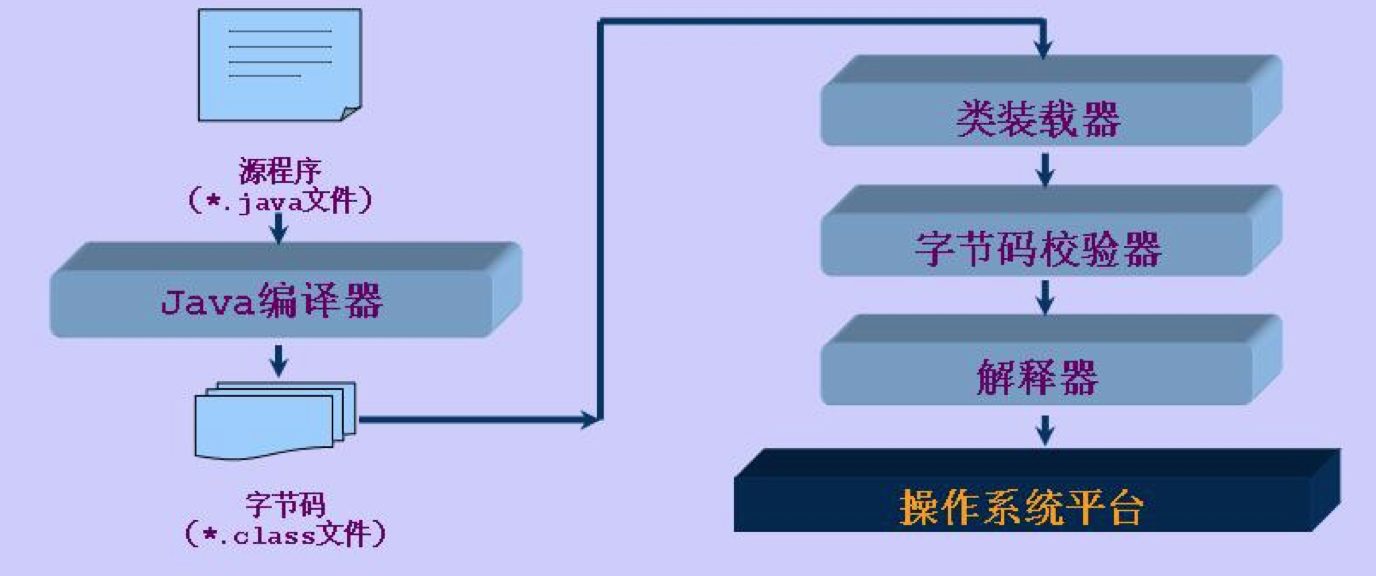
\includegraphics[width=\textwidth]{figures/java_workflow}
\end{frame}

\begin{frame}
  \frametitle{Java虚拟机(JVM)}
  \begin{itemize}
    \item Java源代码编译后形成的字节码无法被操作系统直接执行,只能被JVM执行
    \item JVM可以理解为一个以Java字节码为“机器指令”的虚拟CPU
    \item 不同的操作系统和平台有不同的JVM实现
    \item JVM位于操作系统之上,对其功能进行了封装,以此屏蔽了不同平台底层系统的差异性,实现“一次编译,到处运行”
  \end{itemize}
  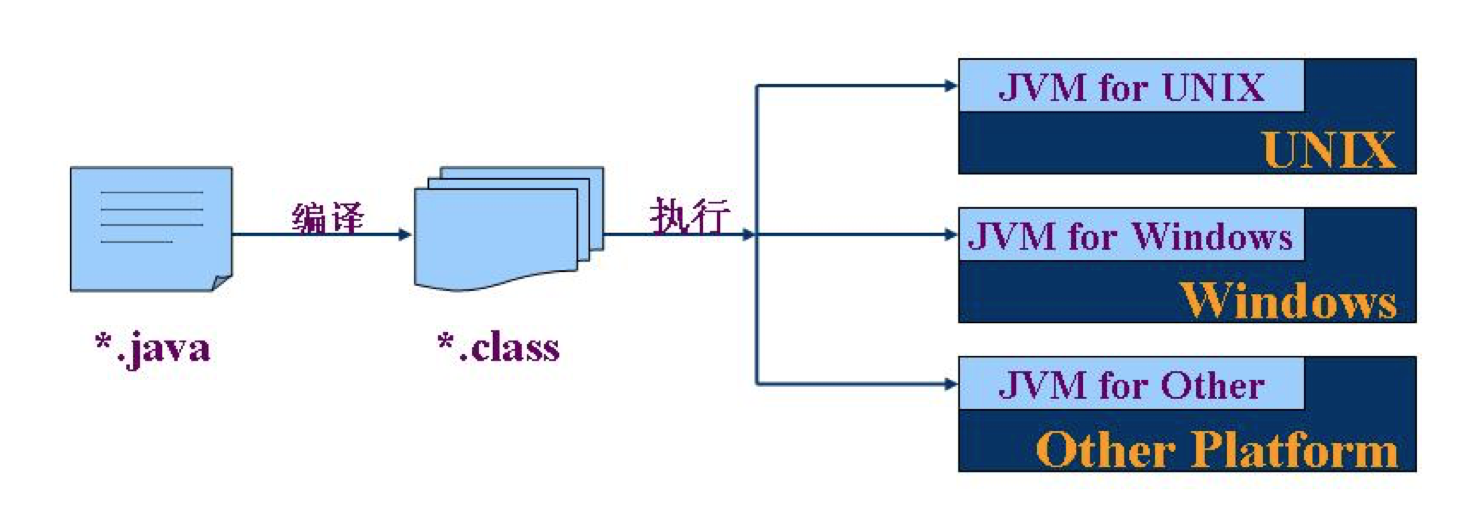
\includegraphics[width=\textwidth]{figures/jvm}

\end{frame}

\begin{frame}
  \frametitle{垃圾收集机制}
  \begin{itemize}
    \item 程序员无需也不能像C/C++中那样手动分配和回收内存(\texttt{malloc}、\texttt{free}等函数)
    \item 不再使用的内存空间会被JVM按照特定算法定期予以释放回收,此过程是JVM自动执行的,程序员无法精准的干预和控制
    \item Java的垃圾回收机制使程序员无需再承担内存管理的责任,有效降低了Java程序设计的复杂度和学习成本
  \end{itemize}
  \begin{block}{\textbf{JVM和垃圾收集带来的“负面影响”}}
    JVM在进行垃圾回收时是需要占用CPU资源的,此时整个JVM中运行的用户线程会停止工作,直到垃圾收集结束,这极大的影响了Java程序的实时性。对于C/C++这种手动管理内存的语言就不存在此问题,因为是程序员负责管理内存。
  \end{block}
\end{frame}

\begin{frame}
  \frametitle{Java发展史}
\begin{table}
\renewcommand\arraystretch{1.4}\arrayrulecolor{LightSteelBlue3}
\begin{tabular}{@{\,}r <{\hskip 2pt} !{\timeline} >{\raggedright\arraybackslash}p{9cm}}
1995 & JDK Beta\\
1996 & JDK 1.0	\\
1998 & J2SE 1.2	\\
2002 & J2SE 1.4	\\
2004 & J2SE 5.0,升级大版本号,直接从1.4升级为5.0\\
2006 & Java SE 6,将J2SE改名为Java SE(还包括Java EE,Java ME) \\
2009 & 年Oracle收购Sun,取得Java所有权\\
2014 & Java SE 8 (LTS,Long Term Support,长支持版本) \\
2018 & Java SE 10 \\
\end{tabular}
\end{table}
\end{frame}

\begin{frame}
  \frametitle{Java平台体系}
    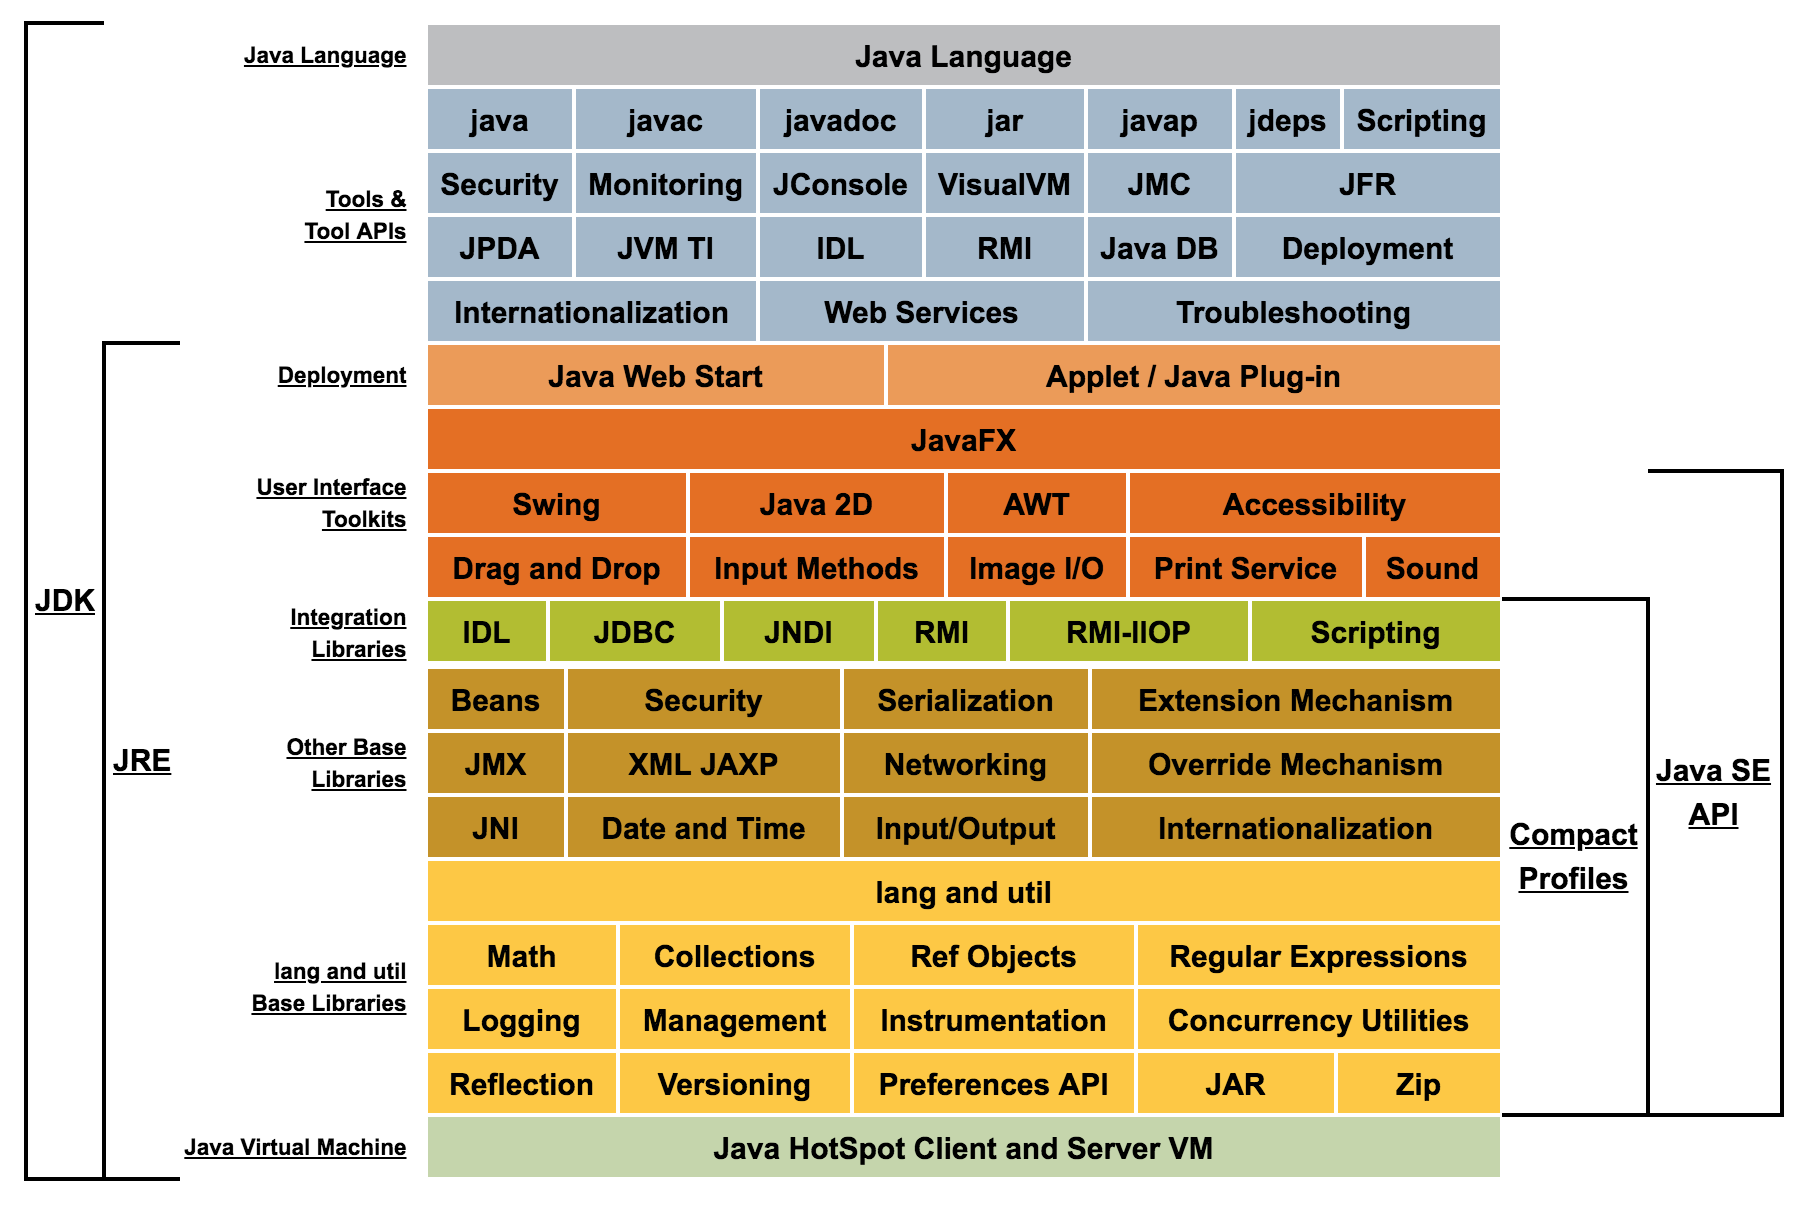
\includegraphics[width=\textwidth]{figures/java_conceptual_diagram}
\end{frame}

\begin{frame}
  \frametitle{Java平台体系中的概念要点}
  \begin{itemize}
    \item JDK和JRE:
      \begin{itemize}
        \item JRE:Java Runtime Environment,包含\textbf{用户运行编译后的Java程序的运行时环境}
        \item JDK:Java Development Kit,包含JRE以及\textbf{Java程序的开发工具包(编译、调试等)}。常用的JDK有官方的Oracle JDK、开源的Open JDK和IBM的J9(现开源为OpenJ9)
        \item 终端用户只需安装JRE即可,只有开发人员才需要安装JDK。JDK安装包较大
      \end{itemize}
    \item Java的版本
      \begin{itemize}
        \item Java ME: Java Micro Edition(逐渐被Android等所取代,用途越来越少,almost dead)
        \item Java SE:Java Standard Edition (主流版本)
        \item Java EE:Java Enterprise Edition(系统过于庞大复杂,应用场景也不多)
      \end{itemize}
  \end{itemize}
\end{frame}



\subsection[第二章:开发环境的搭建]{第二章:开发环境的搭建}
\begin{frame}
  \frametitle{JDK的下载和安装}
  \begin{enumerate}
    \item 利用搜索引擎,找到Oracle JDK的官方下载页面:\href{http://www.oracle.com/technetwork/cn/java/javase/downloads/index.html}{Java SE 下载}
    \item 根据自己操作系统的类型,选择下载对应版本的Java SE 8 JDK
      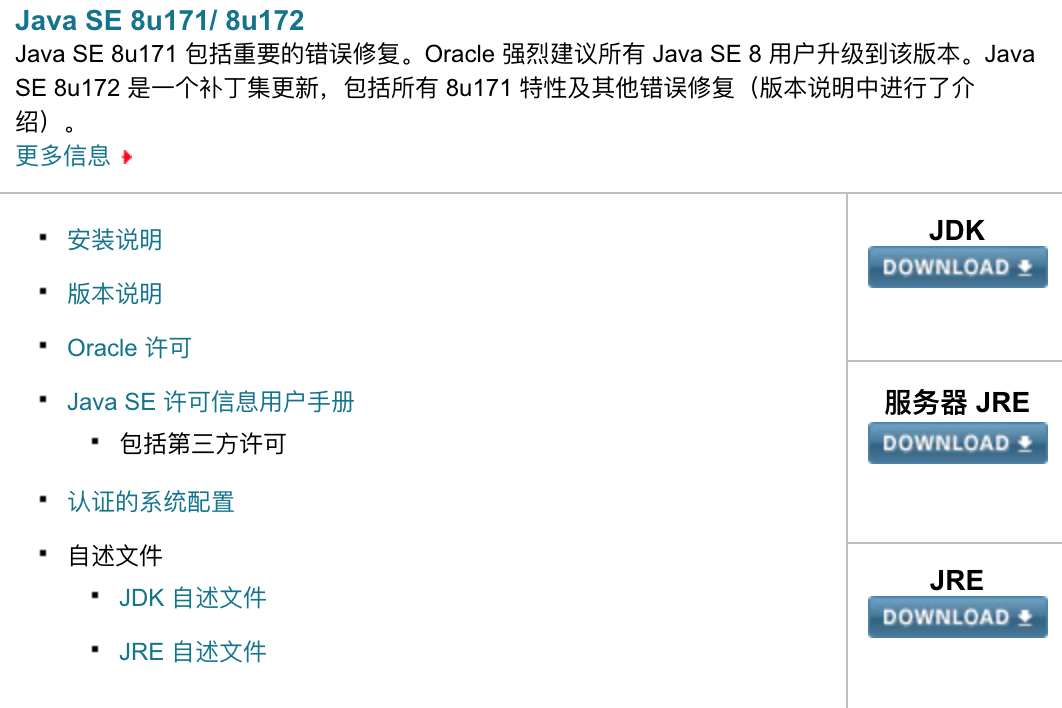
\includegraphics[height=150pt]{figures/oracle_jdk_download}
    \item 双击安装
  \end{enumerate}
\end{frame}

\begin{frame}
  \frametitle{认识JDK}
\end{frame}

\begin{frame}
  \frametitle{设置环境变量(可选)}
  环境变量一般是指在操作系统中用来指定操作系统运行环境的一些参数,这些参数一般以键值对的形式存在。
  
  Windows中可以通过“系统属性”->“高级”选项卡->“环境变量”对话框的方式增加、删除或者编辑修改环境变量。
  \begin{itemize}
    \item 增加\texttt{JAVA\_HOME}环境变量,将其赋值为JDK的安装目录:有些程序凭\texttt{JAVA\_HOME}寻找JDK的安装目录
    \item 修改\texttt{PATH}环境变量,将\texttt{JAVA\_HOME/bin}目录加入:使得可以在任何目录直接使用JDK提供的软件工具,如\texttt{javac}等
  \end{itemize}
  
  \begin{block}{\textbf{环境变量\texttt{PATH}的作用}}
    当你在计算机安装JDK之后,输入\texttt{javac}或者\texttt{java}之类的命令是不能马上被计算机正确执行的,因为计算机不知道到哪里去找这两个命令。那么计算机该如何查找你输入的命令呢? Windows操作系统是根据环境变量\texttt{PATH}来查找命令的。环境变量\texttt{PATH}的值是一系列路径,Windows操作系统将在这一系列的路径中依次查找命令对应的程序文件,如果能找到这个此命令,则该命令是可执行的;否则将出现“‘XXX’不是内部命令或外部命令,也不是可运行的程序或批处理文件”的提示。
  \end{block}
\end{frame}

\begin{frame}
  \frametitle{编写并运行第一个Java程序}
  \begin{enumerate}
    \item 使用任意纯文本编辑器(如记事本、np++等,不要使用Word)编写程序
    \item 使用\texttt{javac}编译程序
    \item 打开命令行窗口,使用\texttt{java}运行程序
  \end{enumerate}
  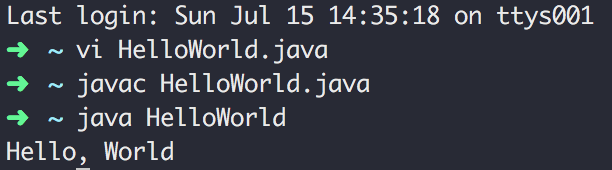
\includegraphics[width=\textwidth*2/3]{figures/hello_world}

\end{frame}

\begin{frame}[fragile]
  \frametitle{程序代码}
  \begin{enumerate}
    \item 右键新建“文本文件”,文件名为\texttt{HelloWorld.java}
    \item 使用记事本打开该文件,并逐行输入如下代码:
    \item 保存文件
  \end{enumerate}
\begin{javacode*}{label=HelloWorld.java}
public class HelloWorld {
   public static void main(String[] args) {
      // Prints "Hello, World"
      System.out.println("Hello, World");
   }
}
\end{javacode*}
\end{frame}

\begin{frame}
  \frametitle{Java源程序代码的基本组织形式}
  \begin{itemize}
    \item 源代码文件必须使用\texttt{.java}做为文件扩展名
    \item 源代码文件名(不包含扩展名)必须和代码中的类名相同!
    \item 源代码严格区分大小写
    \item 如果希望该源代码可以执行,必须定义程序入口函数,函数签名不能改变!\java|public static void main(String[] args)|
  \end{itemize}
  \begin{block}{\textbf{函数签名}}
    函数签名包含了:函数名、函数的参数列表、函数的返回值类型、函数的其他修饰
    \textbf{在Java中,函数也称为“方法”}
  \end{block}

\end{frame}

\begin{frame}
  \frametitle{编译和执行Java程序}
  \begin{enumerate}
    \item 打开命令行,使用\texttt{cd}命令切换到\texttt{HelloWorld.java}所在目录
    \item 编译Java源文件:\texttt{javac HelloWorld.java},得到字节码程序\texttt{HelloWorld}
    \item 执行编译后的字节码程序:\texttt{java HelloWorld},观察屏幕输出
  \end{enumerate}
\end{frame}

\begin{frame}
  \frametitle{代码风格(Code Style)}
  \begin{itemize}
    \item 代码风格又称编码风格、编码规范,是指编写源代码的书写风格,大体包括了:
      \begin{itemize}
        \item 如何给变量、函数、类命名
        \item 如何使用代码缩进
        \item 代码布局,如花括号的摆放位置等
      \end{itemize}
    \item 好的代码风格是出于工程上的要求,没有绝对的对错,只有好坏,代码风格的好坏和不同并不会直接导致程序出错
    \item 好的代码风格可以使得:
      \begin{itemize}
        \item 代码更美观、更加容易阅读理解
        \item 更容易发现编码过程中的错误
      \end{itemize}
    \item 很多人不重视代码风格,认为数学、算法才是根本,或者认为只要代码能运行,怎么书写并不重要。这种思想是错误的!因为正规的现代软件工程已经脱离了一个人小作坊式的编写模式,好的、统一的代码风格有助于提高团队工作效率!
  \end{itemize}
\end{frame}

\begin{frame}[fragile]
  \frametitle{本课程代码风格的要求(一)}
  本课程要求同学们编写代码时,必须遵守如下代码风格(这也是最常见的Java代码风格,参考Google编码风格制定):
  \begin{enumerate}
    \item 变量的命名采用\textbf{小驼峰命名法}:除第一个单词小写之外,其他单词首字母大写,如:\java|int studentCount|
    \item 类的命名采用\textbf{大驼峰命名法}:单词首字母均大写,如: \java|public class HelloWorld|
    \item 静态常量命名全大写,单词之间使用下划线(\texttt{\_})隔开,如: \java|public static final String CONSTANT_PI|
    \item 左花括号写在行末尾,不能新起一行;右花括号独占新的一行书写(也称K \& R 风格),如:
      \begin{javacode}
        public static void main(String[] args) {
        ... ...
        }  
      \end{javacode}
  \end{enumerate}
\end{frame}

\begin{frame}[fragile]
  \frametitle{本课程代码风格的要求(二)}
  \begin{enumerate}
    \setcounter{enumi}{4}
    \item 即使是可选的情况下,也要使用大括号,如:
      \begin{javacode}
        if (count > 6) { //此花括号在语法上可以省略,但是按照我们的代码风格,予以保留
          flag = true; 
        }  
      \end{javacode}
    \item 除非在for循环的定义中,操作符、运算符两边需各有一个空格(做为一个整体的操作符中间不需要加空格,如\texttt{!=}),如:\java|int studentCount = 10 - 1;|
    \item 如果字符的前面是逗号或分号,需要在前加一个空格:\java|for (int a=0; a++; a<10)|
    \item 小括号和中括号前留一个空格,后面不留空格

  \end{enumerate}
\end{frame}

\begin{frame}[fragile]
  \frametitle{本课程代码风格的要求(三)}
  \begin{enumerate}
    \setcounter{enumi}{8}
    \item 采用四个空格或者一个制表符tab做为一个缩进层级
    \item 一行最多只有一个以分号结尾的语句,一行最长100个字符
    \item 不要像C语言那样在函数头部一次性声明很多变量,用到的时候再声明
  \end{enumerate}
  
  \begin{javacode*}{label=错误代码风格举例}
    int a=3; //等号前后需要由空格
    double d = 1.0; double c = 2.0; //一行只应写一个带分号的语句
    public class studentScore {} //类名应该采取大驼峰写法,第一个单词首字母应大写
    static final String numCount; //静态常量应全部使用大写,单词间使用下划线隔开
    String student_name; //变量名应采取小驼峰写法
    
    public void getScore()
    {//此为C的代码风格,本课程中左花括号应写在函数声明行的最后
    return this.score; //此处应该有四个空格或者一个tab的缩进
    } 
  \end{javacode*}

\end{frame}

\begin{frame}[fragile]
  \frametitle{代码注释}
  \begin{columns}
  \column{0.5\textwidth}  
  注释的类型:
\begin{itemize}
  \item 单行注释:
\begin{javacode}
// 我是单行注释!
\end{javacode}
  \item 多行注释:
\begin{javacode}
/* 我是 
* 多行注释!
*/
\end{javacode}
  \item 文档(\texttt{javadoc})注释:
\begin{javacode}
/**
* 演示了文档注释
* @author Ayan Amhed
* @version 1.2
*/
\end{javacode}
\end{itemize}
\column{0.5\textwidth}
为什么必须写注释:
\begin{itemize}
  \item 你的代码可能是要被别人阅读的,别人可能不理解你的逻辑
  \item 你的代码自己以后也要重新阅读,你自己可能也不能理解写作代码当时的逻辑
  \item 写作代码时,帮助自己理清思路
\end{itemize}
\begin{block}{\textbf{注意}}
  注释是程序代码的有机组成部分,一边写代码,一遍写注释。本课程作业要求同学们必须写注释解释自己的思路!
\end{block}
  \end{columns}
\end{frame}

\begin{frame}
  \frametitle{集成开发环境(IDE)}
  \begin{itemize}
    \item IntelliJ IDEA:功能强大,高度集成,易于使用。除了Java也可作为常见绝大多数语言的开发环境
      \begin{itemize}
        \item 社区版(Community):免费使用
        \item 旗舰版(Ultimate):商业使用收费,教育和开源项目免费
      \end{itemize}
    \item Eclipse:功能强大,开源,免费。有多个版本,分别打包了不同的插件,用于Java SE、Java Web等开发
    \item NetBeans:功能强大,开源,免费,使用人数较前两者更少
  \end{itemize}
  
  \begin{block}{\textbf{IDE的选择}}
	\begin{itemize}
		\item 个人开发程序:三种IDE都很成熟,都可以很好的开发Java程序,写不好程序和IDE的选择无关!
		\item 团队开发程序:尽量和团队其他人使用的IDE保持一致
		\item 本课程选择IntelliJ IDEA进行授课,因为该IDE更加遵守Java项目的最佳实践,且大家以后如果学习Android,官方推荐的也是该IDE的衍生产物
	\end{itemize}
  \end{block}

\end{frame}


\section[第二部分:Java语言基础]{第二部分:Java语言基础}
\subsection[第三章:基本数据类型与数组]{第三章:基本数据类型与数组}
\begin{frame}
  \frametitle{关键字}
  \begin{itemize}
    \item 定义:事先定义的,有特别意义的单词,被Java语言保留下来有着特殊含义和用途,所以有时又叫保留字
    \item 所由的Java关键字都是小写
    \item \texttt{goto}和\texttt{const}虽目前未被Java使用,但是依旧是保留关键字
    \item 一般情况下,IDE编辑器会将关键字以特殊高亮的形式展现
  \end{itemize}
  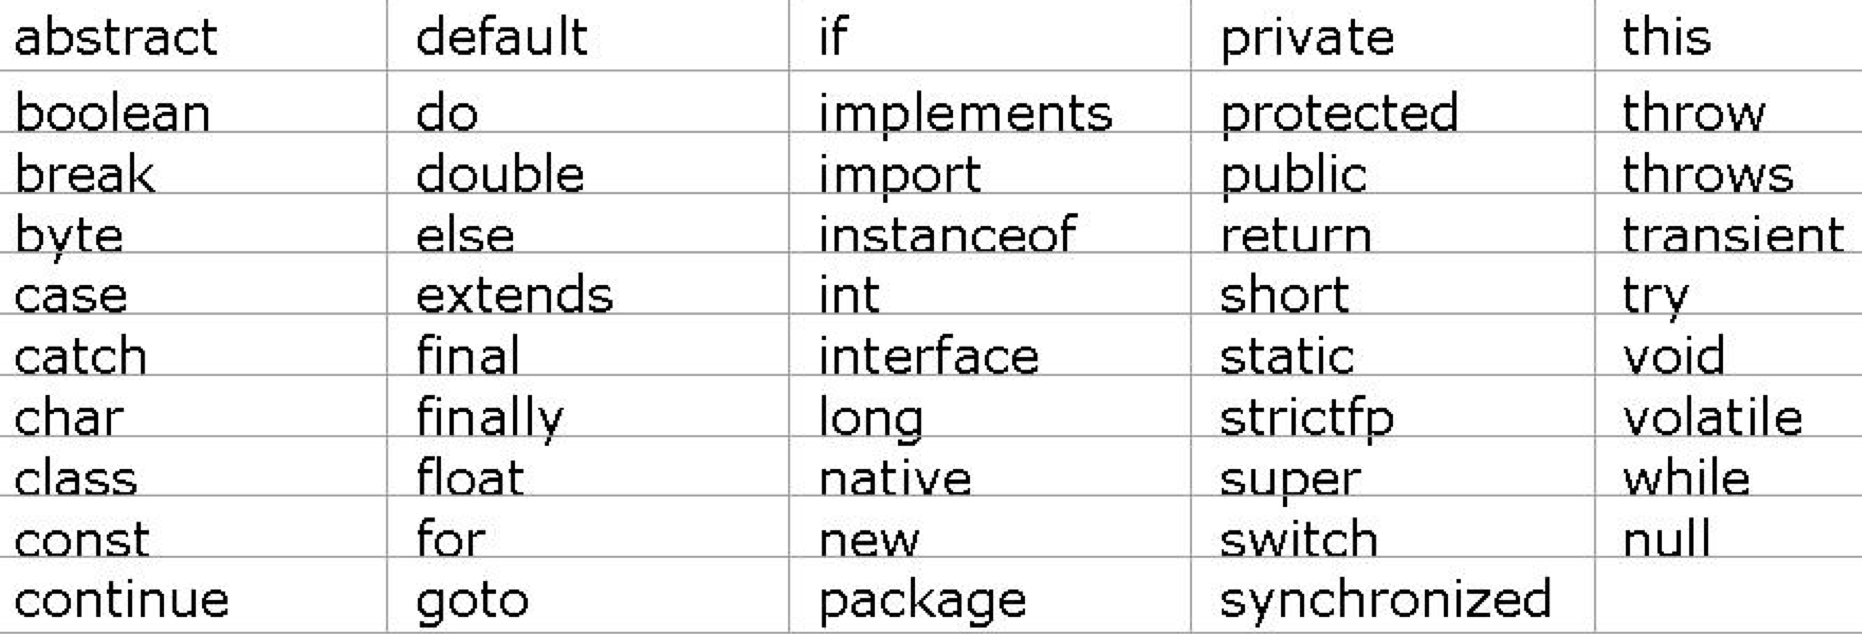
\includegraphics[width=\textwidth]{figures/keywords}
\end{frame}

\begin{frame}
  \frametitle{标识符}
  \begin{itemize}
    \item 定义:用于给Java程序中变量、类、方法等要素命名的字符串序列
    \item Java标识符规则:
      \begin{itemize}
        \item 只能由字母、数字、下划线“\_”、美元符"\$"号组成
        \item 不能以数字开头,只能以字符、下划线、美元符号开头
        \item 不能是Java中的关键字
        \item 大小写敏感
      \end{itemize}
    \item 通俗地说,凡是可以自己起名字的地方,都要遵守标识符规则
    \item 标志符中的字母指Unicode中的字母,不光包括英文26个字母,甚至包括中文的汉字、希腊字母、日文片假名等
    \item 合法标志符举例:\texttt{myName,My\_name,Points,\$points,\_sys\_ta,OK,\_23b,\_3\_}
    \item 非法标志符举例:\texttt{\#name,25name,class,\&time,if}
  \end{itemize}
\end{frame}

\begin{frame}[fragile]
  \frametitle{变量}
  \begin{itemize}
    \item 变量是Java中最基本的数据存储单元,其要素包括:变量名、变量的数据类型和作用域
    \item 变量必须先声明,后使用,声明格式为:\java|type varName [= valValue]|
    \begin{javacode}
      String a; //声明了一个变量,但未赋值,相当于C中的空指针
      int i = 100; //声明了一个变量,并为其赋值
      double a, b, c = 1.1; //一次赋值三个变量
    \end{javacode}
    \item 本质上讲,Java中的变量其实就是内存中的一小块区域,这块区域可以使用变量名来访问
  \end{itemize}
\end{frame}

\begin{frame}
  \frametitle{Java中的数据类型}
  \begin{itemize}
    \item Java中共两大类数据类型:基本数据类型和引用数据类型
    \item 引用数据类型实际就是C语言中的指针引用!Java中除了基本数据类型,其它本质上都是指针!
    \item Java函数的参数如果是基本数据类型,那么传值调用;如果是引用类型,则本质上是传址调用!
  \end{itemize}
  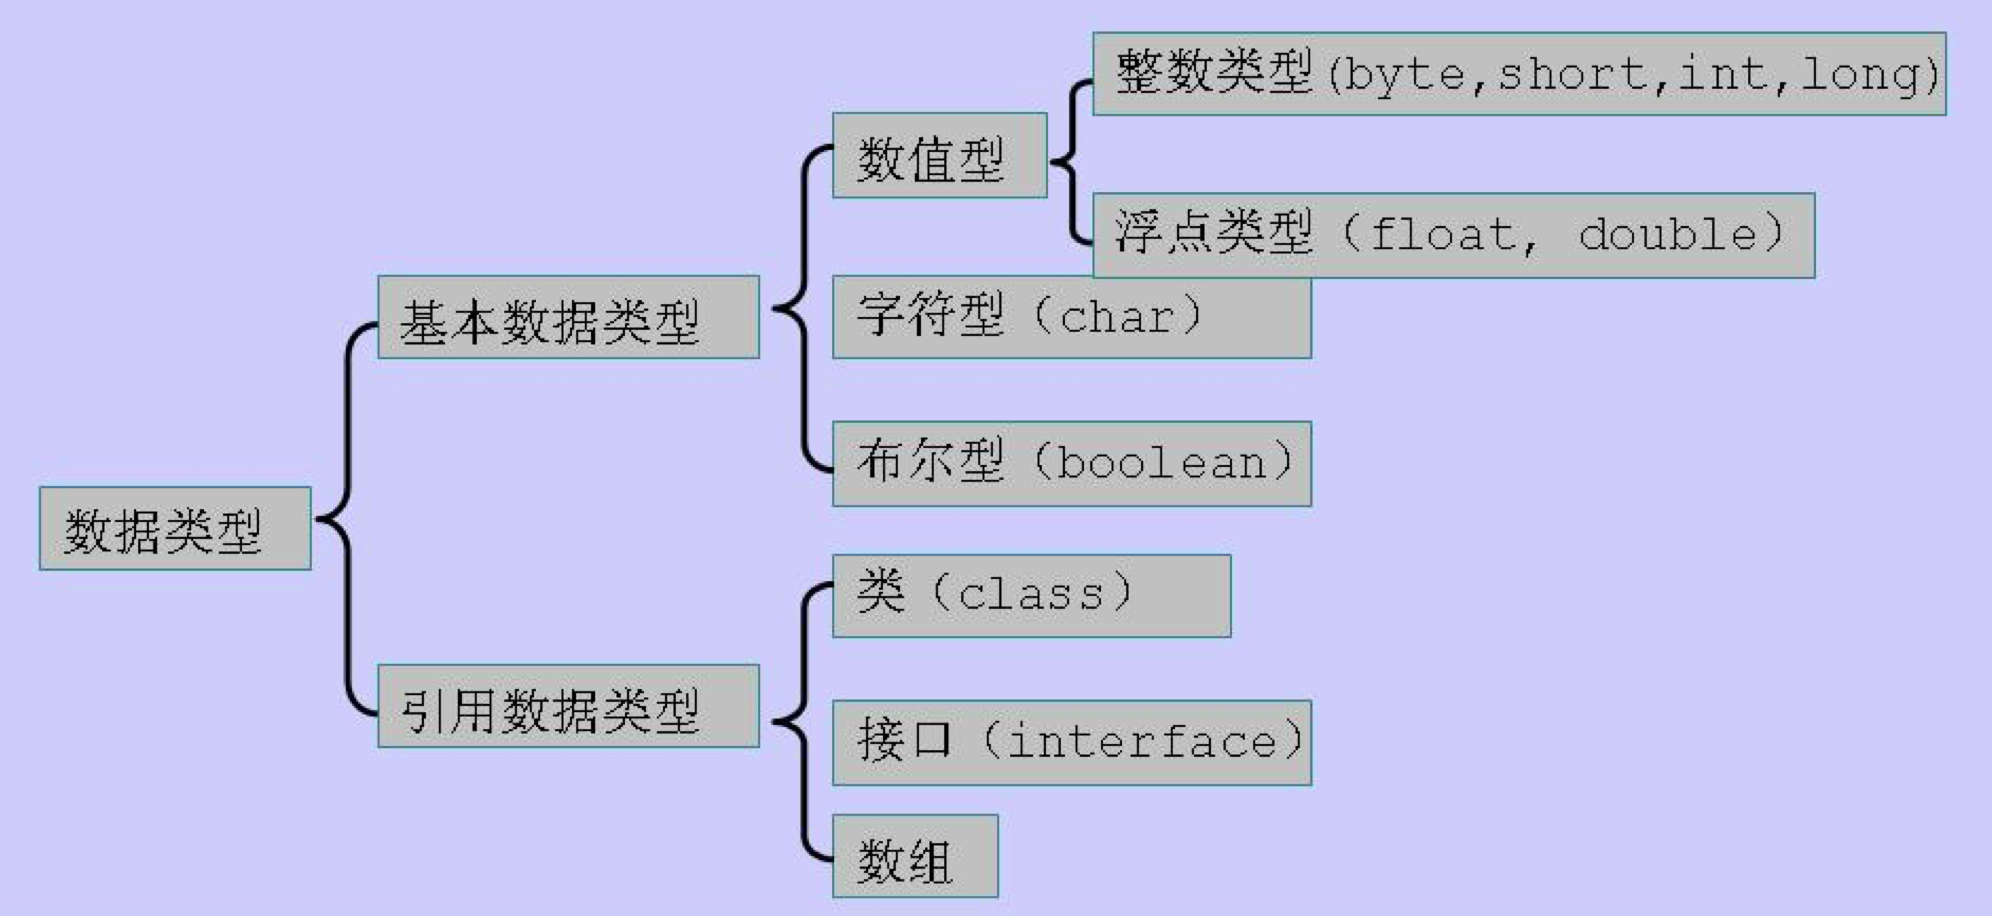
\includegraphics[width=\textwidth]{figures/data_types}
\end{frame}


\begin{frame}[fragile]
  \frametitle{布尔型}
  \begin{itemize}
    \item 布尔型数据用于逻辑运算,一般用于程序流程控制,使用\texttt{boolean}声明一个布尔型变量
    \item Java中的布尔型数据只能取两个值\texttt{true}和\texttt{false},不能使用0或者null来表示(注意此处和和C语言不同)
  \end{itemize}
  \begin{javacode}
    boolean a = true;
    boolean b = false;
    
    if (a) { //使用布尔型数据用于流程控制
    }
    
    boolean c = 0; //错误,Java中布尔型只能取true或者false
    
    int d = -1;
    if (d) { //错误,Java中只能使用布尔型做为程序流程控制
    }
  \end{javacode}
\end{frame}

\begin{frame}[fragile]
  \frametitle{字符型}
  \begin{itemize}
    \item 字符型数据表示一个字符,用单引号\texttt{'}包围(注意不能用双引号,双引号包围的是字符串!)
    \item Java字符采用Unicode编码,每个字符占用两个字节,所以字符类型数据可以转换为整数型数据
    \item Unicode编码的字符不光包含了Asic字符,还包含了很多外语的字母,如汉字等
    \item 允许使用反斜杠来表示具有特殊意义的字符
  \end{itemize}
  \begin{javacode}
    char a = 'x';
    char b = "x"; //错误,双引号括起来的表示字符串
    char c = 'abc'; // 错误,字符型数据只能是1个字符
    char d = '\n'; //表示一个换行符
    char e = '1';// e是一个字符型数据,不是一个整数!
    char f = '中'; //Java中的字是Unicode编码的字符,包括中文
    char f = '\u0061'; // 采用Unicode的形式给字符赋值
  \end{javacode}
\end{frame}

\begin{frame}
  \frametitle{数组}
  \begin{itemize}
    \item 数组是多个\textbf{相同}类型数据的集合
    \item 和C语言中的数组类似,Java中的数组本质上也是一个指针,属于Java的引用类型,做为函数参数是进行传址调用
    \item 声明方式:\java|type valName[]|
  \end{itemize}
\end{frame}

\subsection[第四章:运算符、表达式和语句]{第四章:运算符、表达式和语句}
\begin{frame}[fragile]
  \frametitle{运算符}
  \begin{itemize}
    \item 算术运算符:\texttt{+、-、*、/、\%、++、--}
    \item 关系运算符:\texttt{>、>=、<、<=、==、!=}
    \item 逻辑运算符:\texttt{!、\&\&、||}
    \item 位运算符:\texttt{|,\&,...}
    \item 赋值运算符:\texttt{=}
    \item 扩展赋值运算符:\texttt{+=、-=、*=、/=}
    \item 字符串链接符:\texttt{+}
  \end{itemize}
\end{frame}

\begin{frame}[fragile]
  \frametitle{算术运算符}
  \begin{javacode}
    int m = 6 % 5; //为1,因为余数为1
    int m = 6 % 2; //为0,因为可以整除
    
    int x = 2, y = 2;
    int b = x++; //先赋值,再自增,b=2。计算顺序:b=x, x=x+1
    int c = ++y; //先自增,再赋值,c=3。计算顺序:y=y+1, c=y
    
    3/2; //结果为1!
    
    //Java没有“幂运算符”,通过下述函数完成幂运算
    Math.pow(3, 2); //3的2次方
  \end{javacode}

\end{frame}

\begin{frame}
  \frametitle{逻辑运算符}
  \begin{itemize}
    \item 短路现象        boolean b = (a<4)&&(a++<10);

  \end{itemize}
\end{frame}

\begin{frame}[fragile]
  \frametitle{三目运算}
  \begin{itemize}
    \item 三目运算语法格式:
     \java|x ? y : z|
    \item 解释:其中\texttt{x}为布尔型类型的表达式,如果\texttt{x}为真,则返回\texttt{y};否则,返回\texttt{z}
  \end{itemize}
  
  \begin{javacode}
  int score = 80;
  String type = score > 60 ? "及格" : "不及格"; 
  
  int x = -1;
  int flag =  x > 0 ? 1 : (x == 0 ? 0 : -1)
  // 等价于下列代码:
  if (x > 0) {
    flag = 0;
  } else {
    flag = 1;
  }
  \end{javacode}

\end{frame}

\begin{frame}
  \frametitle{语句}
  \begin{itemize}
    \item 条件语句:根据不同条件,执行不同的代码块
      \java|if|
      \java|if ... else ...|
      \java|if ... else if ... else ...|
      \java|switch ... case ... case ... default ...|
    \item 循环语句:当满足某条件时,重复执行代码块
      \java |for|
      \java |while|
      \java |do ... while ...|
  \end{itemize}

\end{frame}

\begin{frame}[fragile]
  \frametitle{条件语句}
    \begin{columns}
      \column{0.4\textwidth}
        \begin{javacode*}{label=IF语句}
       if (x) {
       
       } 
       
       if (x) {
       
       } else {
       
       }
       
       if (x) {
       
       } else if (y) {
       
       } else {
       
       }
      \end{javacode*}
      \column{0.6\textwidth}
      \begin{javacode*}{label=Switch语句}
        switch(参数) {
          //如果“参数”的值等于“常量表达式1”,则执行
          case 常量表达式1: 
            ...
            break; 
            //不要忘记加break,否则会有副作用
          case 常量表达式2: 
            ...
            break;
          default: 
            break;
        }
      \end{javacode*}
      \begin{itemize}
        \item 小心\texttt{case}穿透,注意加上必要的\texttt{break}
        \item default可以省略,单不推荐
      \end{itemize}
    \end{columns}
\end{frame}


\begin{frame}[fragile]
  \frametitle{FOR循环语句}
  \begin{javacode*}{label=传统形式}
    int[] arr = new int[]{1, 2, 3, 4};
    
    for (int i=0; i< arr.length; i++) {
      System.out.println(x);
    }
  \end{javacode*}
  
  \begin{javacode*}{label=Java 5.0增强形式}
    for (int x in arr) {
      System.out.println(x);
    }
  \end{javacode*}
\end{frame}

\begin{frame}[fragile]
  \frametitle{WHILE循环}
  \begin{columns}
      \column{0.5\textwidth}
        \begin{javacode*}{label=WHILE语句}
          while (逻辑表达式1) {
            代码块1
          }
          //最后没有分号
        \end{javacode*}
        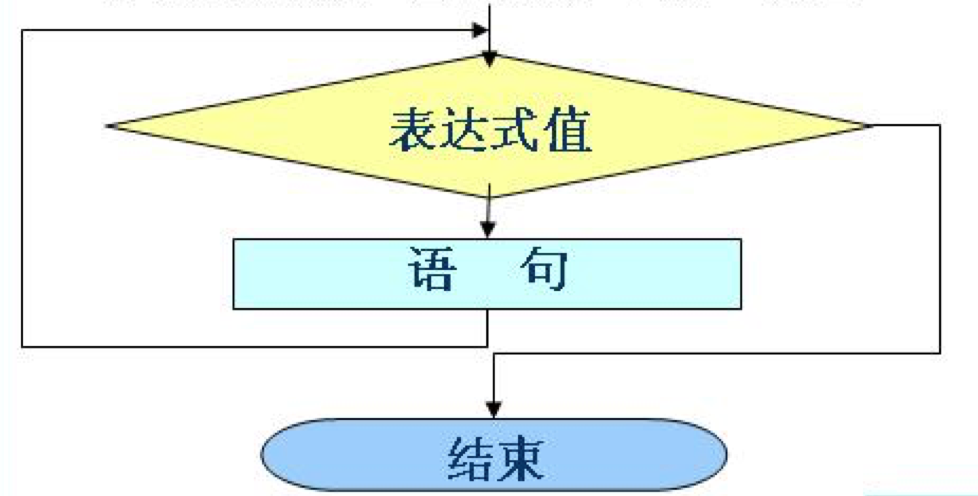
\includegraphics[width=\textwidth, height=80pt]{figures/while}
        当不满足“逻辑表达式1”时,“代码块1”一次都不会执行!
      \column{0.5\textwidth}
        \begin{javacode*}{label=DO WHILE语句}
          do {
            代码块2
          } while (逻辑表达式2); 
          //不要忘记最后有分号
        \end{javacode*}
        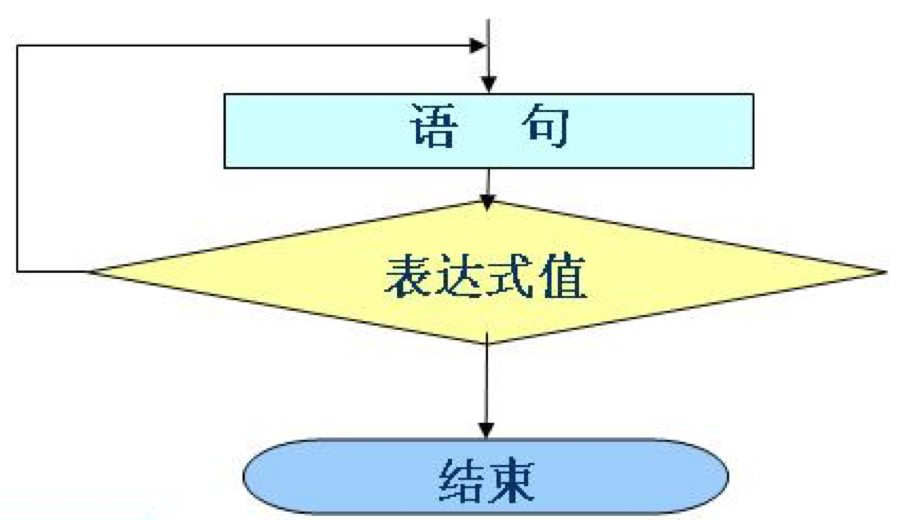
\includegraphics[width=\textwidth, height=80pt]{figures/do_while}
        当不满足“逻辑表达式2”时,“代码块2”会执行1次!
  \end{columns}
    
  \center{如果没有特殊需求,请用第一种WHILE语句!因为第一种WHILE语句意思更明了,更易理解,更加不容易出现副作用!}
\end{frame}

\begin{frame}[fragile]
  \frametitle{循环控制:break语句和continue语句}
    \begin{columns}
      \column{0.5\textwidth}
        break语句用于提前终止循环体的执行,可以强制退出循环,并且不再进行下一轮循环的判定和执行
        \begin{javacode}
        for (int i=0; i< arr.length; i++) { //arr是[1,2,3,4]
          if (i == 3) {
            break;//跳出本循环
          }
          System.out.println(x);
        }
        //只会打印“1, 2”!
        \end{javacode}
      \column{0.5\textwidth}
        continue语句可以提前终止本次循环体的执行,不再执行该语句后面的循环体,开始下一轮循环的判定和执行
        \begin{javacode}
        for (int i=0; i< arr.length; i++) {//arr是[1,2,3,4]
          if (i == 3) {
            continue;//跳出本轮循环
          }
          System.out.println(x);
        }
        //会打印“1, 2, 4”, 不会打印“3”!
        \end{javacode}   
  \end{columns}
  \center{
  \begin{itemize}
    \item 相同点:立即退出本轮循环的循环体,后续循环体的语句都不执行
    \item 不同点:break语句不再进入下一轮的循环判定,而continue语句会进入下一轮的循环判定
  \end{itemize}
  }

\end{frame}

\begin{frame}
  \frametitle{迭代(recursion)}
  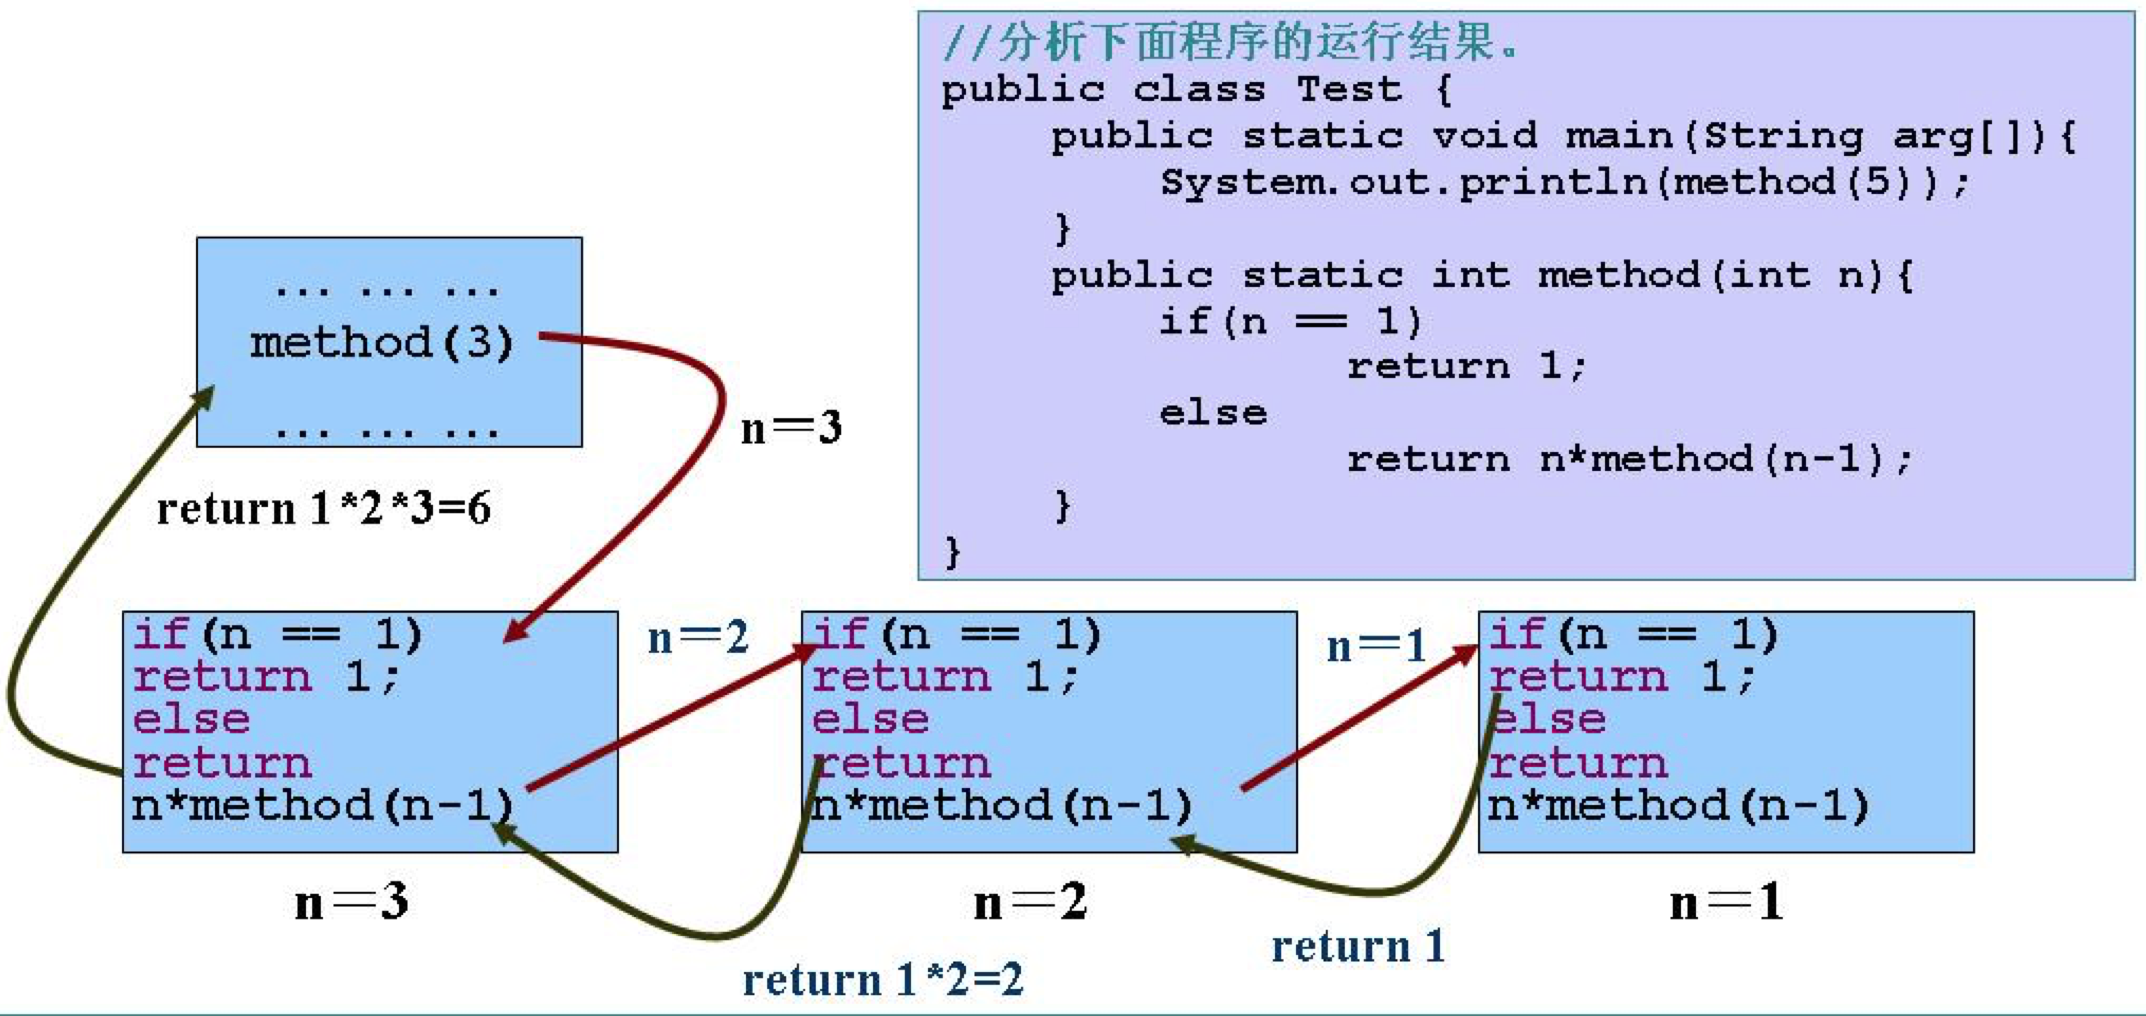
\includegraphics[width=\textwidth]{figures/recursion}
\end{frame}



\section[第三部分:面向对象]{第三部分:面向对象}
\subsection[第五章:面向对象编程]{第五章:面向对象编程}
\begin{frame}
  \frametitle{编程思想}
  \begin{itemize}
    \item 粗略的说,程序=数据结构+算法:
      \begin{itemize}
        \item 数据结构:数据是如何在计算机中存储的
        \item 算法:如何操作数据结构
      \end{itemize}
    \item “编程思想”要\underline{解决的问题}:在软件编程中,如何将真实世界中的复杂事物刻画映射为计算机程序中可编程的数据结构和算法
    \item 目前最为常用的两类编程思想:\underline{面向过程}和\underline{面向对象}
  \end{itemize}
\end{frame}

\begin{frame}
  \frametitle{面向过程编程}
  \begin{itemize}
    \item 面向过程的程序设计把计算机程序视为一系列的命令集合,即一组函数的顺序执行。“过程”就是函数!
    \item “面向过程编程”的\underline{基本思路}:把事物设计为函数,然后把大块函数通过切割成小块函数来降低系统的复杂度。
    \item 程序的设计、编写和运行,本质上都是采用了一种线性的思维
    \item 大家以前学习的C语言就是一门最常见的“面向过程”的编程语言。C语言的入口为主函数\texttt{main},在该函数中调用其它用户设计实现的程序子函数
  \end{itemize}
  \center{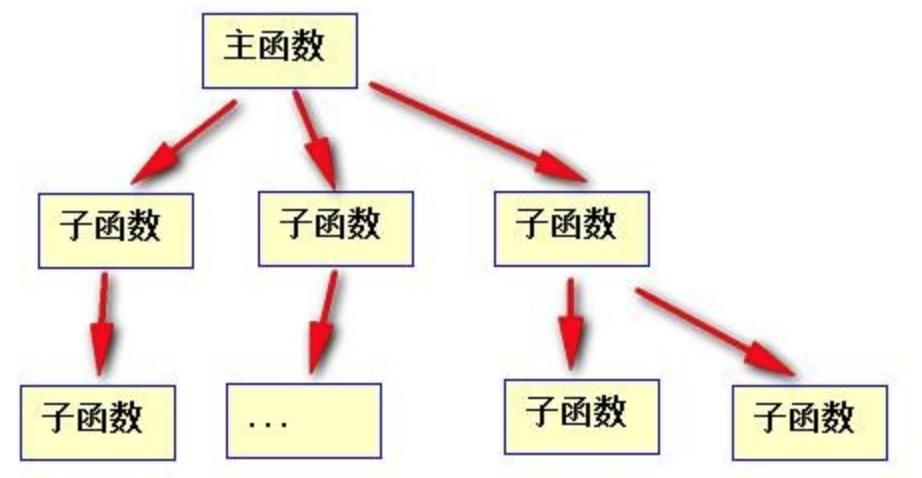
\includegraphics[width=\textwidth/2]{figures/pop}}
\end{frame}

\begin{frame}
  \frametitle{面向对象编程}

    “面向对象编程”(OOP,Object Oriented Programming)的\underline{基本思路}:
    
    将真实世界中的复杂事物抽象、提取、归纳为“对象”
%    \item 把一组数据结构和处理它们的方法组成对象(object),把相同行为的对象归纳为类(class),通过类的封装(encapsulation)隐藏内部细节,通过继承(inheritance)实现类的特化(specialization)/泛化(generalization),通过多态(polymorphism)实现基于对象类型的动态分派(dynamic dispatch)。
  \\
  \\
  举例——历史学家要编写史书,主要有两种形式:
      \begin{itemize}
        \item 纪传史:以人物为中心编写,可以类比为“面向对象”
        \item 编年史:按照事件发生的事件顺序编写,可以类比为“面向过程”
      \end{itemize}

\end{frame}

\begin{frame}
  \frametitle{对象(object)}
  \begin{itemize}
    \item OOP把对象作为程序的基本单元,一个对象包含了:
      \begin{itemize}
        \item 属性:即数据,描述了“该对象有什么数据”
        \item 方法:即操作数据的函数,描述了“该对象能干什么”
      \end{itemize}
    \item 对象=属性(attribute)+方法(method)
    \item 例子一:将“人”这个概念抽象为“对象”
      \begin{itemize}
        \item 属性:姓名、年龄、性别 ...
        \item 方法:吃饭、睡觉、走路 ...
      \end{itemize}
    \item 例子二:将“汽车”这个概念抽象为“对象”
      \begin{itemize}
        \item 属性:发动机、底盘、车身、油箱 ...
        \item 方法:启动、行车、刹车、加油 ...
      \end{itemize}
  \end{itemize}
\end{frame}

\begin{frame}[t]
  \frametitle{面向过程和面向对象在解决问题思路上的差别}
  \center{\textbf{问题:人把大象装冰箱}}
  \vspace{1pt}
  \begin{columns}[t]
    \column{0.4\textwidth}
      \center{\textbf{面向过程的思路}}
      
      \vspace{1pt}
      程序入口主函数:
      \begin{enumerate}
        \item 函数一:打开冰箱
        \item 函数二:把大象塞进去
        \item 函数三:关冰箱门
      \end{enumerate}
    \column{0.6\textwidth}
      \center{\textbf{面向对象的思路}}
      
      \vspace{1pt}
      \underline{设计对象}(只定义了“方法”):
      \begin{itemize}
        \item 人:操作(冰箱),操作(大象)
        \item 大象:进入()
        \item 冰箱:开门(),关门()
      \end{itemize}
       程序入口主函数:
       \begin{enumerate}
         \item 人.操作(冰箱):冰箱.开门()
         \item 人.操作(大象):大象.进入()
         \item 人.操作(冰箱):冰箱.关门()
       \end{enumerate}
  \end{columns}
\end{frame}

\begin{frame}
  \frametitle{类(class)}
  \begin{itemize}
    \item “类”是对一类事物的总结,可以把“类”理解为:对大量对象共性的抽象,是对象的模板。“类”中定义了这一类对象的共有属性和共有方法
    \item “类”具有属性(也称成员变量),它是对象的属性状态的抽象,用数据结构来描述类的属性,人类有姓名、年龄、性别等属性
    \item “类”具有操作(也称方法),它是对象的操作行为的抽象,用操作名和实现该操作的方法来描述,人有吃()、说话()、学习()等方法
    \item “类”的具体化就是对象,也可以说类的实例是对象。如有“人”这个类,统称人类;对象则是具体的某个人,如张三、李四
  \end{itemize}

\end{frame}

\begin{frame}
  \frametitle{类的举例}
  \center{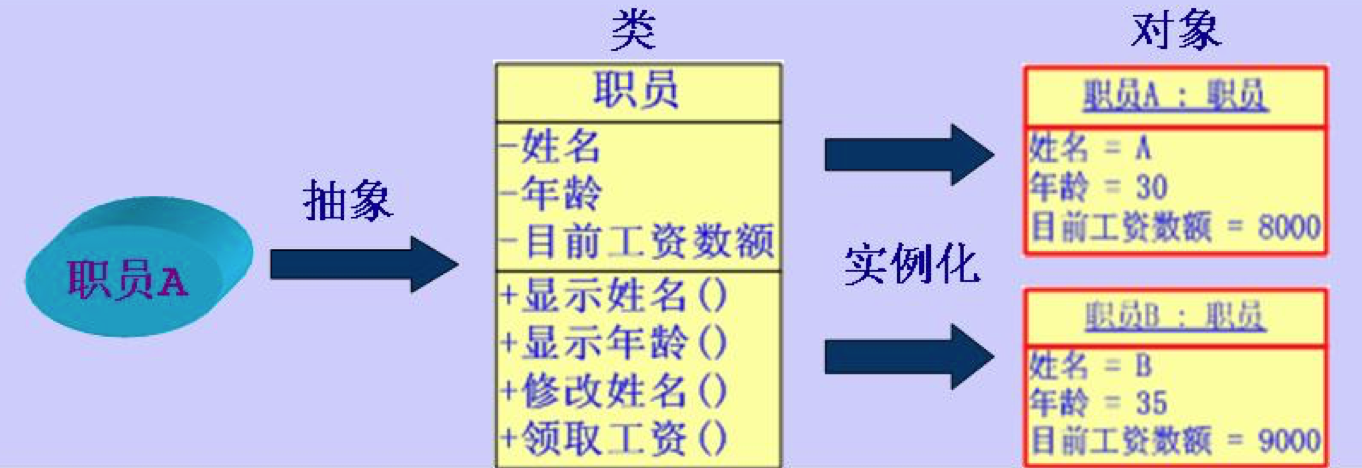
\includegraphics[width=0.8\textwidth]{figures/class_object1}}
  \center{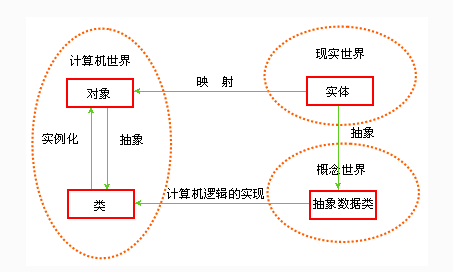
\includegraphics[width=0.7\textwidth]{figures/class_object2}}
\end{frame}

\begin{frame}
  \frametitle{Java中的面向对象编程}
  \begin{itemize}
    \item Java是一门OOP语言\footnote{严格来说,Java只是一门较为纯粹的OOP语言,仍然有一些不属于OOP的元素},在Java中对象是第一公民,程序的设计和编写都是围绕着各种对象展开的
    \item 和Java相对的,C语言这种面相过程的编程语言,函数往往是第一公民
    \item 面向对象的好处:易维护、易复用、易扩展
    \item 在Java中,定义在类中的函数一般称为“方法”
  \end{itemize}
\end{frame}


\subsection[第六章:类与对象]{第六章:类与对象}
\begin{frame}[fragile]
  \frametitle{类的定义}
  \begin{javacode}
  //定义了类:采用驼峰标记
  public class Person {
    //定义成员变量:驼峰标记法
    String id;
    String name;
    int age;
    
    //定义构造方法
    public Person(String fullName, int age) {
      this.fullName = fullName;
      this.age = age;
    }

    //定义方法:驼峰标记法
    void speak(String something) {
      System.out.println(something);
    }
    
  }
  \end{javacode}
\end{frame}

\begin{frame}[fragile]
  \frametitle{类定义中的要点}
  \begin{itemize}
    \item 使用\javainline{class}关键字定义一个类:
      \begin{javacode}
      class 类名 {
        类体
      } //注意,此处没有“;”
      \end{javacode}
    \item \javainline{class} 后面的花括号括住的内容称为“类体”
    \item 代码风格要求:
      \begin{itemize}
        \item 类名采用大驼峰标记
        \item 包围类体的左花括号写在行尾,前面和类名留一个空格,不要新起一行!
        \item 包围类体的右花括号单独新起一行
      \end{itemize}
      \begin{javacode}
        class Test
        {//错误!左花括号应该在上一行的末尾
        }
        class test //错误!类名使用大驼峰标记
      \end{javacode}
  \end{itemize}
\end{frame}

\begin{frame}[fragile]
  \frametitle{成员变量的声明和初始化}
  \begin{itemize}
    \item 对象的属性也称对象的成员变量(member variable,field)
    \item 成员变量是属于对象的,同一个类实例化出的不同对象虽然有着相同类型的成员变量,但是成员变量的赋值却可以不一样
    \item 也即,成员变量的值是绑定在对象上的,而不是类上的
    \item 成员变量的作用域为整个类体
    \item 定义成员变量的方法和定义变量的方法类似:
      \begin{javacode}
        public class Test {
          int a; // 定义一个成员变量
          int b = 2; // 定义一个成员变量,并赋予默认值(也称为初始化)
          private String c; // 成员变量的前部可以加修饰符
        }
      \end{javacode}
  \end{itemize}
\end{frame}

\begin{frame}[fragile]
  \frametitle{成员变量声明中的代码风格}
  \begin{itemize}
    \item 一行只声明一个成员变量
    \item 如果要为成员变量赋予默认值,等号两边要各有一个空格!
    \item 成员变量的命名采用小驼峰标记法
  \end{itemize}
  \begin{javacode}
    public class Test {
      int a; int c;// 错误!一行只推荐定义一个成员变量
      int b=2; // 错误!等号两边需要有空格
      String MyName; // 错误!请使用小驼峰标记法
      String my_name; // 错误!请使用小驼峰标记法
   }
  \end{javacode}
\end{frame}

\begin{frame}[fragile]
  \frametitle{构造函数}
  \begin{itemize}
    \item 构造函数是定义在类体中,用于初始化对象的一种特殊函数,在创建类的对象时,会调用该类的构造函数
    \item 和类体中的一般方法不同,其函数名必须和类名相同,且无需声明返回值类型,也没有返回值(即不能使用\javainline{return}语句)
    \item 当类体中不定义任何构造函数时,Java会为该类自动添加一个默认构造函数。默认构造函数本质是一个无参的、空函数体的构造函数
    \item 当类体中定义了任何一个构造函数时,Java则不会再为该类田间一个默认构造函数
    \item 在类体中可以使用\javainline{this}关键字指代“当前对象本身”,通过\javainline{this}可以调用本对象的所有方法和属性(不管其控制访问修饰符为何):\javainline{this.[方法名或属性名]}
    \item 使用\javainline{this}可以区分同名变量
  \end{itemize}
\end{frame}

\begin{frame}[fragile]
  \frametitle{构造函数举例}
  \begin{javacode}
    public class Person {
      public String name;
      
      //相当于无参构造函数
      public Person(){
      }
      
      //通过构造函数给成员变量进行初始化赋值
      public Person(String name) {
        //this.name指成员变量name,等号右边的name为构造函数的形参
        this.name = name; 
      }
      
      public String getName() {
        return this.name;
      }
    }  
  \end{javacode}
\end{frame}


\begin{frame}
  \frametitle{定义方法}
  \begin{itemize}
    \item 类体中除了构造函数之外的函数称为“方法”
    \item 如果类的方法签名中定义了返回值类型,方法体中最后需要使用\javainline{return}返回
    \item 如果该方法不返回任何值,应该在方法签名中将函数返回值类型设置为\javainline{void}
    \item 代码风格:
      \begin{itemize}
        \item 方法名采用小驼峰命名法
        \item 同类定义中花括号的使用原则一样,方法体的左花括号写在方法签名行的末尾,右花括号新起一行顶头写
        \item 多个形参之间使用逗号隔开时,逗号后面需要有一个空格:\javainline{int add(int x, int y)}
      \end{itemize}
  \end{itemize}
\end{frame}

\begin{frame}[fragile]
  \frametitle{定义方法举例}
  \begin{javacode}
    public class Person {
      public String name;
      
      public String getName() { //有返回值
        return this.name;
      }
      
      public void printName() { //无返回值
        System.out.println(this.name);
      }
      
      public void setName(String name) {
        this.name = name; //直接使用形参
      }
    }  
  \end{javacode}
\end{frame}

\begin{frame}[fragile]
  \frametitle{对象的创建和使用}
  \begin{itemize}
    \item 对象的创建也称为类的实例化
    \item 使用“\javainline{new 构造函数([args])}”的方式创建对象
    \item 使用\javainline{对象.[方法名或属性名]}的方式访问该对象的方法或属性
  \end{itemize}
  \begin{javacode}
    public class Test {
      public static void main(String[] args) {
        Person p = new Person("Jim");
        System.out.println(p.name); //访问对象的属性
        System.out.println(p.getName()); //调用对象的方法
      }
    }
  \end{javacode}

\end{frame}

\begin{frame}
  \frametitle{静态成员变量和静态方法}
\end{frame}

\begin{frame}
  \frametitle{包}
\end{frame}

\begin{frame}
  \frametitle{访问控制修饰符}
  使用访问控制符来保护对类、变量、方法和构造方法的访问:
  \begin{itemize}
    \item \javainline{default}:默认的访问控制符(即缺省,什么也不写),表示在同一包内可见。使用对象:类、接口、变量、方法
    \item \javainline{private}:在同一类内可见。使用对象:变量、方法。不能修饰类(外部类)
    \item \javainline{protected}:对同一包内的类和所有子类可见。使用对象:变量、方法。不能修饰类(外部类)
    \item \javainline{public}:对所有类可见。使用对象:类、接口、变量、方法
  \end{itemize}
\end{frame}

\begin{frame}[fragile]
  \frametitle{访问控制修饰符的应用举例}
  \begin{javacode}
  public class Person {
    private String name = "x";
    public int age = 21;
  }  
  public class Test() {
     public static void main(String[] args) {
        Person p = new Person();
        p.name; //错误!无法从别地类中访问private修饰的属性和方法
        p.age; //正确
      } 
  }
  \end{javacode}

\end{frame}

\begin{frame}
  \frametitle{外部类与内部类}
\end{frame}

\begin{frame}
  \frametitle{对象的创建和使用}
  \begin{itemize}
    \item 必须使用\texttt{new}关键字
  \end{itemize}
\end{frame}

\begin{frame}
  \frametitle{对象的本质}
  \begin{itemize}
    \item 使用\javainline{new}关键字创建类的一个实例对象,本质是在内存中分配一片内存,并将该内存的指针赋值给新创建的对象变量
    \item 除了基本类型外,所有Java中的对象,本质上都是指针
    \item 所以Java中方法的形参,如果是基本类型,则为传值调用,如果为对象,则为传址调用!
  \end{itemize}
\end{frame}



\subsection[第七章:子类与继承]{第七章:子类与继承}
\subsection[第八章:接口与实现]{第八章:接口与实现}
\subsection[第九章:泛型]{第九章:泛型}

\section[第四部分:实用功能]{第四部分:实用功能}
\subsection[第十章:常用工具类]{第十章:常用工具类}
\input{10_utilities}

\subsection[第十一章:容器类]{第十一章:容器类}
\begin{frame}
  \frametitle{主要类别}
  \begin{itemize}
    \item 列表:\texttt{List},数据的一维有序集合
    \item 集合:\texttt{Set},类似列表,但是集合容器内没有重复的元素
    \item 哈希表:\texttt{Map},表示键值对
  \end{itemize}
\end{frame}

\begin{frame}
  \frametitle{x}
\end{frame}

\begin{frame}
  \frametitle{列表List}
  实现了\texttt{List}的主要容器类:
  \begin{itemize}
    \item \texttt{ArrayList}:内部使用数组实现,但是长度可变
    \item \texttt{LinkedList}:内部使用链表结构实现,可以快速的在某一位置删除和插入元素
  \end{itemize}
\end{frame}

\begin{frame}
  \frametitle{List的主要方法}
   \begin{itemize}
    \item \javainline{boolean add(E e)}:添加元素
    \item \javainline{boolean add(int index, E e)}:在指定位置添加元素
    \item \javainline{E set(int index, E e)}:将指位置的元素替换为新元素
    \item \javainline{boolean get(int index)}:取得指位置的元素
    \item \javainline{int indexOf(E e)}:获得元素在容器里的位置
    \item \javainline{boolean remove(int index)}:删除指位置的元素
    \item \javainline{boolean remove(E e)}:删除制定元素
    \item \javainline{boolean removeAll(Collection c)}:从本容器中删除\texttt{c}中指定的所有元素
    \item \javainline{void clear()}:清空本容器
    \item \javainline{void toArray()}:转换为数组
  \end{itemize}

\end{frame}

\begin{frame}
  \frametitle{ArrayList}
\end{frame}

\begin{frame}
  \frametitle{LinkedList}
\end{frame}

\begin{frame}
  \frametitle{哈希表Map}
  实现了\texttt{Map}的主要容器类:
  \begin{itemize}
    \item \texttt{HashMap}:不保证键值对之间的有序性
    \item \texttt{LinkedHashMap}:保证键值对可以保持插入顺序
  \end{itemize}
\end{frame}

\begin{frame}[fragile]
  \frametitle{Map的主要方法}
  \begin{itemize}
    \item \javainline{V get(K key)}:根据\texttt{key}取出一个与之对应的值
    \item \javainline{V put(K key, V value)}:插入一个键值对
    \item \javainline{V remove()}:根据\texttt{key}取出一个元素
    \item \javainline{boolean containsKey(K key)}:移除容器内键为\texttt{key}对应的键值对
    \item \javainline{int size()}:返回容器内键值对的数目
    \item \javainline{boolean isEmpty()}:返回容器是否为空
    \item \javainline{void putAll(map)}:将参数map中的所有键值对插入本容器
    \item \javainline{Set<Map.Entry> entrySet()}:以\texttt{Set}的方式取出容器内所有的键值对,方便遍历
  \end{itemize}
\end{frame}

\begin{frame}[fragile]
  \frametitle{HashMap}

\end{frame}

\begin{frame}[fragile]
  \frametitle{LinkedHashMap}

\end{frame}

\begin{frame}
  \frametitle{Set}
  定义为包含了不重复的元素集合,主要实现类为\texttt{HashSet},主要方法包括:
  \begin{itemize}
    \item \javainline{boolean add(E e)}:
    \item \javainline{boolean contains(E e)}:
    \item \javainline{boolean isEmpty()}:
    \item \javainline{boolean remove(E e)}:
    \item \javainline{boolean removeAll(collection)}:
    \item \javainline{void clear()}:
    \item \javainline{void toArray()}:
  \end{itemize}
\end{frame}

\begin{frame}
  \frametitle{HashSet}
\end{frame}

\begin{frame}
  \frametitle{LinkedList}
\end{frame}



\subsection[第十二章:输入输出流]{第十二章:输入输出流}

\section[第五部分:高级功能]{第五部分:高级功能}
\subsection[第十三章:多线程技术]{第十三章:多线程技术}
\subsection[第十四章:基于Socket的网络编程]{第十四章:基于Socket的网络编程}
\subsection[第十五章:反射机制]{第十五章:反射机制}



\end{document}